\documentclass[a4paper,11pt]{article}

% Kodovani (cestiny) v dokumentu: utf-8
%\usepackage[cp1250]{inputenc}	% Omezena stredoevropska kodova stranka, pouze MSW.
\usepackage[utf8]{inputenc}	% Doporucujeme pouzivat UTF-8 (unicode).

\usepackage[margin=2cm]{geometry}
\newtoks\jmenopraktika \newtoks\jmeno \newtoks\datum
\newtoks\obor \newtoks\skupina \newtoks\rocnik \newtoks\semestr
\newtoks\cisloulohy \newtoks\jmenoulohy
\newtoks\tlak \newtoks\teplota \newtoks\vlhkost

\jmenopraktika={Fyzikální praktikum 2}
\jmeno={Lukáš Lejdar}
\datum={26. listopadu 2024}
\obor={F}
\skupina={Út 16:00}

\cisloulohy={2}
\jmenoulohy={Charakteristiky tranzistoru a tranzistor jako zesilovač napětí}

\tlak={100{,}5}
\teplota={21,3}
\vlhkost={47}


%%%%%%%%%%% Uzitecne balicky:
\usepackage[czech]{babel}

\usepackage{graphicx}
\usepackage{amsmath}
\usepackage{xspace}
\usepackage{url}
\usepackage{indentfirst}
\usepackage{wrapfig}
\usepackage{xcolor}
\usepackage{subfig}
\usepackage{subcaption}
\usepackage{enumitem}
\usepackage{tikzsymbols}
\usepackage{newfloat}

\DeclareFloatingEnvironment[fileext=lof]{graph}
\captionsetup[graph]{labelformat=simple, labelsep=colon, name=Graf}

%%%%%% Zamezeni parchantu:
\widowpenalty 10000 \clubpenalty 10000 \displaywidowpenalty 10000
%%%%%% Parametry pro moznost vsazeni vetsiho poctu obrazku na stranku
\setcounter{topnumber}{3}	  % max. pocet floatu nahore (specifikace t)
\setcounter{bottomnumber}{3}	  % max. pocet floatu dole (specifikace b)
\setcounter{totalnumber}{6}	  % max. pocet floatu na strance celkem
\renewcommand\topfraction{0.9}	  % max podil stranky pro floaty nahore
\renewcommand\bottomfraction{0.9} % max podil stranky pro floaty dole
\renewcommand\textfraction{0.1}	  % min podil stranky, ktery musi obsahovat text
\intextsep=8mm \textfloatsep=8mm  %\intextsep pro ulozeni [h] floatu a \textfloatsep pro [b] or [t]

% Tecky za cisly sekci:
\renewcommand{\thesection}{\arabic{section}.}
\renewcommand{\thesubsection}{\thesection\arabic{subsection}.}
% Jednopismenna mezera mezi cislem a nazvem kapitoly:
\makeatletter \def\@seccntformat#1{\csname the#1\endcsname\hspace{1ex}} \makeatother
%
\newcommand{\vsn}[4]{\ensuremath{#1 =} #2(#3)\,#4}
\newcommand{\vrn}[6]{\ensuremath{#1 =} (#2 $\pm$ #3)\,#4 ($p=$ #5\,\%, $\nu=$ #6)}

\newcommand*\circled[1]{\tikz[baseline=(char.base)]{
		\node[shape=circle,draw,inner sep=1pt] (char) {#1};}}

%%%%%%%%%%%%%%%%%%%%%%%%%%%%%%%%%%%%%%%%%%%%%%%%%%%%%%%%%%%%%%%%%%%%%%%%%%%%%%%
% Zacatek dokumentu
%%%%%%%%%%%%%%%%%%%%%%%%%%%%%%%%%%%%%%%%%%%%%%%%%%%%%%%%%%%%%%%%%%%%%%%%%%%%%%%

\begin{document}

\thispagestyle{empty}

{
\begin{center}
\sf 
{\Large Ústav fyziky a technologií plazmatu Přírodovědecké fakulty Masarykovy univerzity} \\
\bigskip
{\huge \bfseries FYZIKÁLNÍ PRAKTIKUM} \\
\bigskip
{\Large \the\jmenopraktika}
\end{center}

\bigskip

\sf
\noindent
\setlength{\arrayrulewidth}{1pt}
\begin{tabular*}{\textwidth}{@{\extracolsep{\fill}} l l}
\large {\bfseries Zpracoval:}  \the\jmeno & \large  {\bfseries Naměřeno:} \the\datum\\[2mm]
\large  {\bfseries Obor:} \the\obor  \hspace{40mm}  {\bfseries Skupina:} \the\skupina %
&\large {\bfseries Testováno:}\\
\\
\hline
\end{tabular*}
}

\bigskip

{
\sf
\noindent \begin{tabular}{p{4cm} p{0.6\textwidth}}
\Large  Úloha č. {\bfseries \the\cisloulohy:} \par
\smallskip
$T=\the\teplota$~$^\circ$C \par
$p=\the\tlak$~kPa \par
$\varphi=\the\vlhkost$~\%
&\Large \bfseries \the\jmenoulohy  \\[2mm]
\end{tabular}
}

\vskip1cm

\section{Úvod}

V úloze budu měřit charakteristiky unipolárního tranzistoru ve zvoleném pracovním bodě a v druhé části ho zapojím jako zesilovač napětí. Několika způsoby potom určím toto zesílení.

\section{Postup měření}

\subsection{Výstupní a převodní charakteristika transistoru}

 Proud $ I_D $  tekoucí transistorem mezi jeho svorkami $ S $ (Source) a $ D $ (Drain) je určený hradlovým napětím $ U_G $ a napětím $ U_D $ mezi svorkami $ S $ a $ D $. 

 \begin{equation}
 I_D = f(U_D, U_G)
 \end{equation}

 Pro měření této závislosti použiju obvod jako na obrázku 1. Na zdroji vlevo se nastavuje napětí $ U_G $ a zdroj vpravo řídí napětí $ U_D $, které způsobí proud tekoucí ze svorky D skrz Ampermetr. Účelem kontaktů $ +S $ a $ -S $ je udržovat stejné napětí jako mezi kontakty + a -, aby nebylo potřeba počítat s vnitřním odporem Ampermetru.

\begin{figure}[htpb]
    \centering
    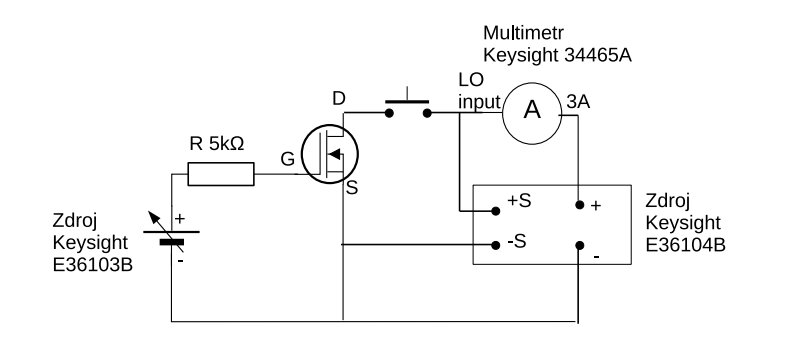
\includegraphics[width=0.65\textwidth]{charakteristiky_schema.jpg}
    \caption{Zapojení pro měření charakteristik}
\end{figure}


 Pokud se bude tranzistor používat jen v okolí některého pracovního bodu $ (U_{D0}, U_{G0}) $, je běžné funkci $ f $ aproximovat lineárně veličinami

\begin{align}
    S = \frac{\partial I_D}{\partial U_G}(U_{D0}, U_{G0}) && R_i = \frac{\partial U_D}{\partial I_D}(U_{D0}, U_{G0}).
\end{align}

$ R_i $  je potom vnitřní odpor tranzistoru a $ S $ se nazývá statická strmost. Další veličina, která se zavádí je zesilovací činitel

\begin{equation}
\mu = \frac{\partial U_D}{\partial U_G} \Big |_{I_D = konst.}
\end{equation}

\noindent
který se dá spočítat jako

\begin{equation}
\mu = S R_i
\end{equation}

Zvolím si některý pracovní bod $ (U_{D0}, U_{G0}) $ a změřím charakteristiky $ f(U_{D0}, U_{G}) $  a $ f(U_{D}, U_{G0}) $ , ze kterých dopočítám zmíněné parametry.


\subsection{Tranzistor jako zesilovač napětí}

Na obrázku 2 je návrh obvodu pro zesílení vstupu $ U_1 $ střídavého nebo stejnosměrného napětí na výstup $ U_2 $. Před měřením je ale potřeba na zesilovači nastavit napětí $ E $ a zatěžovací odpor $ R_z $ v závislosti na pracovním bodě. Pro můj účel bude dobré použít $ E =  $ 20 V a $ R_z $ dopočítám z

\begin{equation}
 R_z = \frac{E - U_{D0}}{I_{D0}}
\end{equation}

Po nastavení zesilovače zapnu generátor střídavého napětí $ U_{1} $ a budu měřit napětí na kolektoru $ U_{2} $ . Zesílení signálu je v takovém případě definované amplitudami jako

\begin{equation}
    A_M = \frac{U_{m2}}{U_{m1}}
\end{equation}

Teoreticky je toto zesílení vlastně jen úplná derivace $ U_D $ podle $ U_G $. Jde odvodit, že zároveň platí

\begin{equation}
A_D = \frac{d U_D}{d U_G} = \frac{-\mu}{1 + \frac{R_i}{R_z}} = -S_d Rz 
\end{equation}

\begin{equation}
S_d = \frac{dI_D}{dU_G} = \frac{S}{1 + \frac{R_z}{R_i}}
\end{equation}

Tuto derivaci můžu aproximovat i z měření v 1. části, pokud z grafů správně odečtu podle zatěžovací přímky (5) pro proměnné $ I_D $ a $ U_D $.

\begin{equation}
A = \frac{\Delta U_D}{\Delta U_G}
\end{equation}

\begin{figure}[htpb]
    \centering
    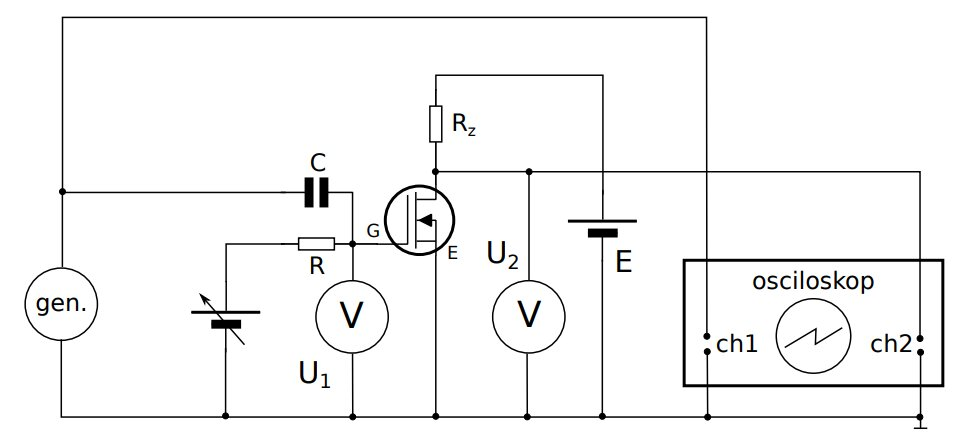
\includegraphics[width=0.55\textwidth]{zesilovac.jpg}
    \caption{Schéma zapojení pro měření vlastností zesilovače}
\end{figure}


\newpage

\section{Výsledky měření}

\subsection{Výstupní a převodní charakteristika transistoru}

Sestavil jsem obvod podle obrázku 1 a změřil výstupní a převodní charakteristiku transistoru pro pracovní bod $ (U_{D0}, U_{G0}) = ( 10 \ V, 3.6 \ V ) $. To stejné měření jsem ještě jednou provedl přesněji za pomoci počítače a výsledky vynesl do grafů 1, 2 a 3. Z lineárního fitu v okolí pracovního bodu jsem získal hodnoty

\begin{align*}
    I_{D0} &= 7.063 \text{ mA} \\
    R_i &=  18.9 \pm 2.8 \ \text{k}\Omega \\
    S &= 0.0617 \pm 0.0041 \ \Omega^{-1} \\
    \mu &= (1.17 \pm 0.19) \cdot 10^{3} \\ 
\end{align*}

\begin{table}[htpb]
    \begin{minipage}[b]{.5\linewidth}
        \centering
        % GNUPLOT: LaTeX picture with Postscript
\begingroup
  \makeatletter
  \providecommand\color[2][]{%
    \GenericError{(gnuplot) \space\space\space\@spaces}{%
      Package color not loaded in conjunction with
      terminal option `colourtext'%
    }{See the gnuplot documentation for explanation.%
    }{Either use 'blacktext' in gnuplot or load the package
      color.sty in LaTeX.}%
    \renewcommand\color[2][]{}%
  }%
  \providecommand\includegraphics[2][]{%
    \GenericError{(gnuplot) \space\space\space\@spaces}{%
      Package graphicx or graphics not loaded%
    }{See the gnuplot documentation for explanation.%
    }{The gnuplot epslatex terminal needs graphicx.sty or graphics.sty.}%
    \renewcommand\includegraphics[2][]{}%
  }%
  \providecommand\rotatebox[2]{#2}%
  \@ifundefined{ifGPcolor}{%
    \newif\ifGPcolor
    \GPcolorfalse
  }{}%
  \@ifundefined{ifGPblacktext}{%
    \newif\ifGPblacktext
    \GPblacktexttrue
  }{}%
  % define a \g@addto@macro without @ in the name:
  \let\gplgaddtomacro\g@addto@macro
  % define empty templates for all commands taking text:
  \gdef\gplbacktext{}%
  \gdef\gplfronttext{}%
  \makeatother
  \ifGPblacktext
    % no textcolor at all
    \def\colorrgb#1{}%
    \def\colorgray#1{}%
  \else
    % gray or color?
    \ifGPcolor
      \def\colorrgb#1{\color[rgb]{#1}}%
      \def\colorgray#1{\color[gray]{#1}}%
      \expandafter\def\csname LTw\endcsname{\color{white}}%
      \expandafter\def\csname LTb\endcsname{\color{black}}%
      \expandafter\def\csname LTa\endcsname{\color{black}}%
      \expandafter\def\csname LT0\endcsname{\color[rgb]{1,0,0}}%
      \expandafter\def\csname LT1\endcsname{\color[rgb]{0,1,0}}%
      \expandafter\def\csname LT2\endcsname{\color[rgb]{0,0,1}}%
      \expandafter\def\csname LT3\endcsname{\color[rgb]{1,0,1}}%
      \expandafter\def\csname LT4\endcsname{\color[rgb]{0,1,1}}%
      \expandafter\def\csname LT5\endcsname{\color[rgb]{1,1,0}}%
      \expandafter\def\csname LT6\endcsname{\color[rgb]{0,0,0}}%
      \expandafter\def\csname LT7\endcsname{\color[rgb]{1,0.3,0}}%
      \expandafter\def\csname LT8\endcsname{\color[rgb]{0.5,0.5,0.5}}%
    \else
      % gray
      \def\colorrgb#1{\color{black}}%
      \def\colorgray#1{\color[gray]{#1}}%
      \expandafter\def\csname LTw\endcsname{\color{white}}%
      \expandafter\def\csname LTb\endcsname{\color{black}}%
      \expandafter\def\csname LTa\endcsname{\color{black}}%
      \expandafter\def\csname LT0\endcsname{\color{black}}%
      \expandafter\def\csname LT1\endcsname{\color{black}}%
      \expandafter\def\csname LT2\endcsname{\color{black}}%
      \expandafter\def\csname LT3\endcsname{\color{black}}%
      \expandafter\def\csname LT4\endcsname{\color{black}}%
      \expandafter\def\csname LT5\endcsname{\color{black}}%
      \expandafter\def\csname LT6\endcsname{\color{black}}%
      \expandafter\def\csname LT7\endcsname{\color{black}}%
      \expandafter\def\csname LT8\endcsname{\color{black}}%
    \fi
  \fi
    \setlength{\unitlength}{0.0500bp}%
    \ifx\gptboxheight\undefined%
      \newlength{\gptboxheight}%
      \newlength{\gptboxwidth}%
      \newsavebox{\gptboxtext}%
    \fi%
    \setlength{\fboxrule}{0.5pt}%
    \setlength{\fboxsep}{1pt}%
    \definecolor{tbcol}{rgb}{1,1,1}%
\begin{picture}(5040.00,2880.00)%
    \gplgaddtomacro\gplbacktext{%
      \csname LTb\endcsname%%
      \put(682,320){\makebox(0,0)[r]{\strut{}$0$}}%
      \put(682,788){\makebox(0,0)[r]{\strut{}$2$}}%
      \put(682,1256){\makebox(0,0)[r]{\strut{}$4$}}%
      \put(682,1723){\makebox(0,0)[r]{\strut{}$6$}}%
      \put(682,2191){\makebox(0,0)[r]{\strut{}$8$}}%
      \put(682,2659){\makebox(0,0)[r]{\strut{}$10$}}%
      \put(938,-134){\makebox(0,0){\strut{}$0$}}%
      \put(1432,-134){\makebox(0,0){\strut{}$2$}}%
      \put(1926,-134){\makebox(0,0){\strut{}$4$}}%
      \put(2420,-134){\makebox(0,0){\strut{}$6$}}%
      \put(2914,-134){\makebox(0,0){\strut{}$8$}}%
      \put(3408,-134){\makebox(0,0){\strut{}$10$}}%
      \put(3902,-134){\makebox(0,0){\strut{}$12$}}%
      \put(4396,-134){\makebox(0,0){\strut{}$14$}}%
      \put(3043,2333){\makebox(0,0)[l]{\strut{}}}%
      \csname LTb\endcsname%%
      \put(3189,2179){\makebox(0,0)[l]{\strut{}$p$}}%
    }%
    \gplgaddtomacro\gplfronttext{%
      \csname LTb\endcsname%%
      \put(209,1372){\rotatebox{-270.00}{\makebox(0,0){\strut{}$ I_D $ (mA)}}}%
      \put(2728,-464){\makebox(0,0){\strut{}$ U_D $ (V)}}%
    }%
    \gplbacktext
    \put(0,0){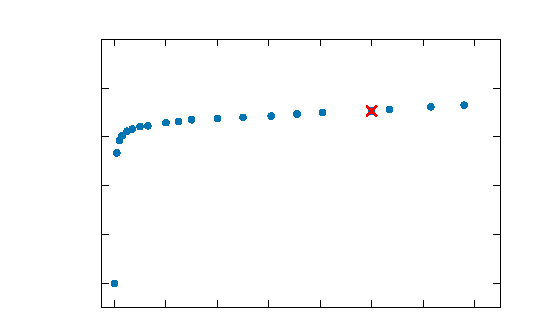
\includegraphics[width={252.00bp},height={144.00bp}]{vystupni_3V6}}%
    \gplfronttext
  \end{picture}%
\endgroup

        \captionsetup{type=graph, justification=centering}
        \caption{Výstupní charakteristika pro \\ $ U_G = 3.6 $ V }
    \end{minipage} 
    \begin{minipage}[b]{.5\linewidth}
        \centering
        % GNUPLOT: LaTeX picture with Postscript
\begingroup
  \makeatletter
  \providecommand\color[2][]{%
    \GenericError{(gnuplot) \space\space\space\@spaces}{%
      Package color not loaded in conjunction with
      terminal option `colourtext'%
    }{See the gnuplot documentation for explanation.%
    }{Either use 'blacktext' in gnuplot or load the package
      color.sty in LaTeX.}%
    \renewcommand\color[2][]{}%
  }%
  \providecommand\includegraphics[2][]{%
    \GenericError{(gnuplot) \space\space\space\@spaces}{%
      Package graphicx or graphics not loaded%
    }{See the gnuplot documentation for explanation.%
    }{The gnuplot epslatex terminal needs graphicx.sty or graphics.sty.}%
    \renewcommand\includegraphics[2][]{}%
  }%
  \providecommand\rotatebox[2]{#2}%
  \@ifundefined{ifGPcolor}{%
    \newif\ifGPcolor
    \GPcolorfalse
  }{}%
  \@ifundefined{ifGPblacktext}{%
    \newif\ifGPblacktext
    \GPblacktexttrue
  }{}%
  % define a \g@addto@macro without @ in the name:
  \let\gplgaddtomacro\g@addto@macro
  % define empty templates for all commands taking text:
  \gdef\gplbacktext{}%
  \gdef\gplfronttext{}%
  \makeatother
  \ifGPblacktext
    % no textcolor at all
    \def\colorrgb#1{}%
    \def\colorgray#1{}%
  \else
    % gray or color?
    \ifGPcolor
      \def\colorrgb#1{\color[rgb]{#1}}%
      \def\colorgray#1{\color[gray]{#1}}%
      \expandafter\def\csname LTw\endcsname{\color{white}}%
      \expandafter\def\csname LTb\endcsname{\color{black}}%
      \expandafter\def\csname LTa\endcsname{\color{black}}%
      \expandafter\def\csname LT0\endcsname{\color[rgb]{1,0,0}}%
      \expandafter\def\csname LT1\endcsname{\color[rgb]{0,1,0}}%
      \expandafter\def\csname LT2\endcsname{\color[rgb]{0,0,1}}%
      \expandafter\def\csname LT3\endcsname{\color[rgb]{1,0,1}}%
      \expandafter\def\csname LT4\endcsname{\color[rgb]{0,1,1}}%
      \expandafter\def\csname LT5\endcsname{\color[rgb]{1,1,0}}%
      \expandafter\def\csname LT6\endcsname{\color[rgb]{0,0,0}}%
      \expandafter\def\csname LT7\endcsname{\color[rgb]{1,0.3,0}}%
      \expandafter\def\csname LT8\endcsname{\color[rgb]{0.5,0.5,0.5}}%
    \else
      % gray
      \def\colorrgb#1{\color{black}}%
      \def\colorgray#1{\color[gray]{#1}}%
      \expandafter\def\csname LTw\endcsname{\color{white}}%
      \expandafter\def\csname LTb\endcsname{\color{black}}%
      \expandafter\def\csname LTa\endcsname{\color{black}}%
      \expandafter\def\csname LT0\endcsname{\color{black}}%
      \expandafter\def\csname LT1\endcsname{\color{black}}%
      \expandafter\def\csname LT2\endcsname{\color{black}}%
      \expandafter\def\csname LT3\endcsname{\color{black}}%
      \expandafter\def\csname LT4\endcsname{\color{black}}%
      \expandafter\def\csname LT5\endcsname{\color{black}}%
      \expandafter\def\csname LT6\endcsname{\color{black}}%
      \expandafter\def\csname LT7\endcsname{\color{black}}%
      \expandafter\def\csname LT8\endcsname{\color{black}}%
    \fi
  \fi
    \setlength{\unitlength}{0.0500bp}%
    \ifx\gptboxheight\undefined%
      \newlength{\gptboxheight}%
      \newlength{\gptboxwidth}%
      \newsavebox{\gptboxtext}%
    \fi%
    \setlength{\fboxrule}{0.5pt}%
    \setlength{\fboxsep}{1pt}%
    \definecolor{tbcol}{rgb}{1,1,1}%
\begin{picture}(5040.00,2880.00)%
    \gplgaddtomacro\gplbacktext{%
      \csname LTb\endcsname%%
      \put(682,284){\makebox(0,0)[r]{\strut{}$0$}}%
      \put(682,680){\makebox(0,0)[r]{\strut{}$10$}}%
      \put(682,1076){\makebox(0,0)[r]{\strut{}$20$}}%
      \put(682,1471){\makebox(0,0)[r]{\strut{}$30$}}%
      \put(682,1867){\makebox(0,0)[r]{\strut{}$40$}}%
      \put(682,2263){\makebox(0,0)[r]{\strut{}$50$}}%
      \put(682,2659){\makebox(0,0)[r]{\strut{}$60$}}%
      \put(814,-134){\makebox(0,0){\strut{}$0$}}%
      \put(1293,-134){\makebox(0,0){\strut{}$0.5$}}%
      \put(1771,-134){\makebox(0,0){\strut{}$1$}}%
      \put(2250,-134){\makebox(0,0){\strut{}$1.5$}}%
      \put(2729,-134){\makebox(0,0){\strut{}$2$}}%
      \put(3207,-134){\makebox(0,0){\strut{}$2.5$}}%
      \put(3686,-134){\makebox(0,0){\strut{}$3$}}%
      \put(4164,-134){\makebox(0,0){\strut{}$3.5$}}%
      \put(4643,-134){\makebox(0,0){\strut{}$4$}}%
      \put(3895,924){\makebox(0,0)[l]{\strut{}}}%
      \csname LTb\endcsname%%
      \put(4041,770){\makebox(0,0)[l]{\strut{}$p$}}%
    }%
    \gplgaddtomacro\gplfronttext{%
      \csname LTb\endcsname%%
      \put(209,1372){\rotatebox{-270.00}{\makebox(0,0){\strut{}$I_D$ (mA)}}}%
      \put(2728,-464){\makebox(0,0){\strut{}$U_G$ (V)}}%
    }%
    \gplbacktext
    \put(0,0){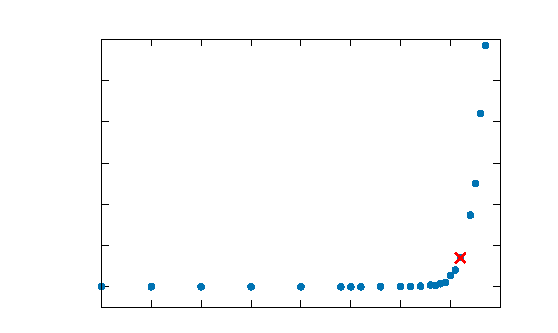
\includegraphics[width={252.00bp},height={144.00bp}]{prevodni_10V}}%
    \gplfronttext
  \end{picture}%
\endgroup

        \captionsetup{type=graph, justification=centering}
        \caption{Převodní charakteristika pro \\ $ U_D = 10 $ V }
    \end{minipage} 
\end{table}

\begin{figure}[htpb]
    \centering
    % GNUPLOT: LaTeX picture with Postscript
\begingroup
  \makeatletter
  \providecommand\color[2][]{%
    \GenericError{(gnuplot) \space\space\space\@spaces}{%
      Package color not loaded in conjunction with
      terminal option `colourtext'%
    }{See the gnuplot documentation for explanation.%
    }{Either use 'blacktext' in gnuplot or load the package
      color.sty in LaTeX.}%
    \renewcommand\color[2][]{}%
  }%
  \providecommand\includegraphics[2][]{%
    \GenericError{(gnuplot) \space\space\space\@spaces}{%
      Package graphicx or graphics not loaded%
    }{See the gnuplot documentation for explanation.%
    }{The gnuplot epslatex terminal needs graphicx.sty or graphics.sty.}%
    \renewcommand\includegraphics[2][]{}%
  }%
  \providecommand\rotatebox[2]{#2}%
  \@ifundefined{ifGPcolor}{%
    \newif\ifGPcolor
    \GPcolorfalse
  }{}%
  \@ifundefined{ifGPblacktext}{%
    \newif\ifGPblacktext
    \GPblacktexttrue
  }{}%
  % define a \g@addto@macro without @ in the name:
  \let\gplgaddtomacro\g@addto@macro
  % define empty templates for all commands taking text:
  \gdef\gplbacktext{}%
  \gdef\gplfronttext{}%
  \makeatother
  \ifGPblacktext
    % no textcolor at all
    \def\colorrgb#1{}%
    \def\colorgray#1{}%
  \else
    % gray or color?
    \ifGPcolor
      \def\colorrgb#1{\color[rgb]{#1}}%
      \def\colorgray#1{\color[gray]{#1}}%
      \expandafter\def\csname LTw\endcsname{\color{white}}%
      \expandafter\def\csname LTb\endcsname{\color{black}}%
      \expandafter\def\csname LTa\endcsname{\color{black}}%
      \expandafter\def\csname LT0\endcsname{\color[rgb]{1,0,0}}%
      \expandafter\def\csname LT1\endcsname{\color[rgb]{0,1,0}}%
      \expandafter\def\csname LT2\endcsname{\color[rgb]{0,0,1}}%
      \expandafter\def\csname LT3\endcsname{\color[rgb]{1,0,1}}%
      \expandafter\def\csname LT4\endcsname{\color[rgb]{0,1,1}}%
      \expandafter\def\csname LT5\endcsname{\color[rgb]{1,1,0}}%
      \expandafter\def\csname LT6\endcsname{\color[rgb]{0,0,0}}%
      \expandafter\def\csname LT7\endcsname{\color[rgb]{1,0.3,0}}%
      \expandafter\def\csname LT8\endcsname{\color[rgb]{0.5,0.5,0.5}}%
    \else
      % gray
      \def\colorrgb#1{\color{black}}%
      \def\colorgray#1{\color[gray]{#1}}%
      \expandafter\def\csname LTw\endcsname{\color{white}}%
      \expandafter\def\csname LTb\endcsname{\color{black}}%
      \expandafter\def\csname LTa\endcsname{\color{black}}%
      \expandafter\def\csname LT0\endcsname{\color{black}}%
      \expandafter\def\csname LT1\endcsname{\color{black}}%
      \expandafter\def\csname LT2\endcsname{\color{black}}%
      \expandafter\def\csname LT3\endcsname{\color{black}}%
      \expandafter\def\csname LT4\endcsname{\color{black}}%
      \expandafter\def\csname LT5\endcsname{\color{black}}%
      \expandafter\def\csname LT6\endcsname{\color{black}}%
      \expandafter\def\csname LT7\endcsname{\color{black}}%
      \expandafter\def\csname LT8\endcsname{\color{black}}%
    \fi
  \fi
    \setlength{\unitlength}{0.0500bp}%
    \ifx\gptboxheight\undefined%
      \newlength{\gptboxheight}%
      \newlength{\gptboxwidth}%
      \newsavebox{\gptboxtext}%
    \fi%
    \setlength{\fboxrule}{0.5pt}%
    \setlength{\fboxsep}{1pt}%
    \definecolor{tbcol}{rgb}{1,1,1}%
\begin{picture}(6480.00,3600.00)%
    \gplgaddtomacro\gplbacktext{%
      \csname LTb\endcsname%%
      \put(682,435){\makebox(0,0)[r]{\strut{}$0$}}%
      \put(682,1089){\makebox(0,0)[r]{\strut{}$10$}}%
      \put(682,1744){\makebox(0,0)[r]{\strut{}$20$}}%
      \put(682,2398){\makebox(0,0)[r]{\strut{}$30$}}%
      \put(682,3052){\makebox(0,0)[r]{\strut{}$40$}}%
      \put(1091,-112){\makebox(0,0){\strut{}$0$}}%
      \put(1646,-112){\makebox(0,0){\strut{}$2$}}%
      \put(2201,-112){\makebox(0,0){\strut{}$4$}}%
      \put(2755,-112){\makebox(0,0){\strut{}$6$}}%
      \put(3310,-112){\makebox(0,0){\strut{}$8$}}%
      \put(3864,-112){\makebox(0,0){\strut{}$10$}}%
      \put(4419,-112){\makebox(0,0){\strut{}$12$}}%
      \put(4974,-112){\makebox(0,0){\strut{}$14$}}%
      \put(5528,-112){\makebox(0,0){\strut{}$16$}}%
      \put(6083,-112){\makebox(0,0){\strut{}$18$}}%
      \put(3499,1258){\makebox(0,0)[l]{\strut{}$(U_{D0}, U_{G0})$}}%
    }%
    \gplgaddtomacro\gplfronttext{%
      \csname LTb\endcsname%%
      \put(5096,2832){\makebox(0,0)[r]{\strut{}$U_G = 3.8$ V}}%
      \csname LTb\endcsname%%
      \put(5096,2612){\makebox(0,0)[r]{\strut{}$U_G = 3.7$ V}}%
      \csname LTb\endcsname%%
      \put(5096,2392){\makebox(0,0)[r]{\strut{}$U_G = 3.6$ V}}%
      \csname LTb\endcsname%%
      \put(5096,2172){\makebox(0,0)[r]{\strut{}$U_G = 3.5$ V}}%
      \csname LTb\endcsname%%
      \put(5096,1952){\makebox(0,0)[r]{\strut{}$U_G = 3.4$ V}}%
      \csname LTb\endcsname%%
      \put(209,1743){\rotatebox{-270.00}{\makebox(0,0){\strut{}$ I_D $ (mA)}}}%
      \put(3448,-442){\makebox(0,0){\strut{}$ U_D $ (V)}}%
    }%
    \gplbacktext
    \put(0,0){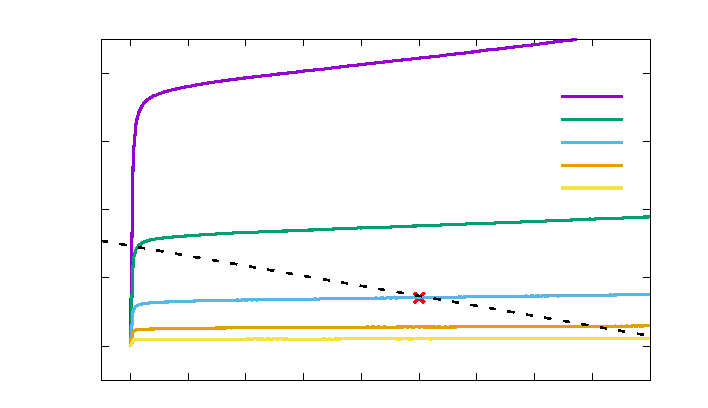
\includegraphics[width={324.00bp},height={180.00bp}]{charakteristiky}}%
    \gplfronttext
  \end{picture}%
\endgroup

    \captionsetup{type=graph}
    \caption{Automatické měření výstupních charakteristik}
\end{figure}

\subsection{Tranzistor jako zesilovač napětí}

Sestavil jsem obvod podle obrázku 2 a pro několik vstupních napětí $ U_{m1} $ měřil zesílený signál $ U_{m2} $. Amplitudy jsou vynesené do grafu (4) a fit je přímkou, jejíž sklon je zesílení $ A_M $. Toto zesílení jsem potom počítal i podle vztahu (7) z hodnot z první části měření a taky odečtením z grafu (3), kde se zatěžovací přímka protíná se sousedními hladinamy $ U_G = 3.7 $ V a $ U_G = 3.5 $ V.

\begin{align*}
   A_M &= 77.5 \pm 0.6 \\
   A_G &= 80.5 \pm 2 \\
   A_V &= 78 \pm 4 \\
   S_d &= 0.058 \pm 0.004 \ \Omega^{-1} \\
\end{align*}

\begin{figure}[htpb]
    \centering
    % GNUPLOT: LaTeX picture with Postscript
\begingroup
  \makeatletter
  \providecommand\color[2][]{%
    \GenericError{(gnuplot) \space\space\space\@spaces}{%
      Package color not loaded in conjunction with
      terminal option `colourtext'%
    }{See the gnuplot documentation for explanation.%
    }{Either use 'blacktext' in gnuplot or load the package
      color.sty in LaTeX.}%
    \renewcommand\color[2][]{}%
  }%
  \providecommand\includegraphics[2][]{%
    \GenericError{(gnuplot) \space\space\space\@spaces}{%
      Package graphicx or graphics not loaded%
    }{See the gnuplot documentation for explanation.%
    }{The gnuplot epslatex terminal needs graphicx.sty or graphics.sty.}%
    \renewcommand\includegraphics[2][]{}%
  }%
  \providecommand\rotatebox[2]{#2}%
  \@ifundefined{ifGPcolor}{%
    \newif\ifGPcolor
    \GPcolorfalse
  }{}%
  \@ifundefined{ifGPblacktext}{%
    \newif\ifGPblacktext
    \GPblacktexttrue
  }{}%
  % define a \g@addto@macro without @ in the name:
  \let\gplgaddtomacro\g@addto@macro
  % define empty templates for all commands taking text:
  \gdef\gplbacktext{}%
  \gdef\gplfronttext{}%
  \makeatother
  \ifGPblacktext
    % no textcolor at all
    \def\colorrgb#1{}%
    \def\colorgray#1{}%
  \else
    % gray or color?
    \ifGPcolor
      \def\colorrgb#1{\color[rgb]{#1}}%
      \def\colorgray#1{\color[gray]{#1}}%
      \expandafter\def\csname LTw\endcsname{\color{white}}%
      \expandafter\def\csname LTb\endcsname{\color{black}}%
      \expandafter\def\csname LTa\endcsname{\color{black}}%
      \expandafter\def\csname LT0\endcsname{\color[rgb]{1,0,0}}%
      \expandafter\def\csname LT1\endcsname{\color[rgb]{0,1,0}}%
      \expandafter\def\csname LT2\endcsname{\color[rgb]{0,0,1}}%
      \expandafter\def\csname LT3\endcsname{\color[rgb]{1,0,1}}%
      \expandafter\def\csname LT4\endcsname{\color[rgb]{0,1,1}}%
      \expandafter\def\csname LT5\endcsname{\color[rgb]{1,1,0}}%
      \expandafter\def\csname LT6\endcsname{\color[rgb]{0,0,0}}%
      \expandafter\def\csname LT7\endcsname{\color[rgb]{1,0.3,0}}%
      \expandafter\def\csname LT8\endcsname{\color[rgb]{0.5,0.5,0.5}}%
    \else
      % gray
      \def\colorrgb#1{\color{black}}%
      \def\colorgray#1{\color[gray]{#1}}%
      \expandafter\def\csname LTw\endcsname{\color{white}}%
      \expandafter\def\csname LTb\endcsname{\color{black}}%
      \expandafter\def\csname LTa\endcsname{\color{black}}%
      \expandafter\def\csname LT0\endcsname{\color{black}}%
      \expandafter\def\csname LT1\endcsname{\color{black}}%
      \expandafter\def\csname LT2\endcsname{\color{black}}%
      \expandafter\def\csname LT3\endcsname{\color{black}}%
      \expandafter\def\csname LT4\endcsname{\color{black}}%
      \expandafter\def\csname LT5\endcsname{\color{black}}%
      \expandafter\def\csname LT6\endcsname{\color{black}}%
      \expandafter\def\csname LT7\endcsname{\color{black}}%
      \expandafter\def\csname LT8\endcsname{\color{black}}%
    \fi
  \fi
    \setlength{\unitlength}{0.0500bp}%
    \ifx\gptboxheight\undefined%
      \newlength{\gptboxheight}%
      \newlength{\gptboxwidth}%
      \newsavebox{\gptboxtext}%
    \fi%
    \setlength{\fboxrule}{0.5pt}%
    \setlength{\fboxsep}{1pt}%
    \definecolor{tbcol}{rgb}{1,1,1}%
\begin{picture}(5760.00,2880.00)%
    \gplgaddtomacro\gplbacktext{%
      \csname LTb\endcsname%%
      \put(682,86){\makebox(0,0)[r]{\strut{}$2$}}%
      \put(682,372){\makebox(0,0)[r]{\strut{}$4$}}%
      \put(682,658){\makebox(0,0)[r]{\strut{}$6$}}%
      \put(682,944){\makebox(0,0)[r]{\strut{}$8$}}%
      \put(682,1230){\makebox(0,0)[r]{\strut{}$10$}}%
      \put(682,1515){\makebox(0,0)[r]{\strut{}$12$}}%
      \put(682,1801){\makebox(0,0)[r]{\strut{}$14$}}%
      \put(682,2087){\makebox(0,0)[r]{\strut{}$16$}}%
      \put(682,2373){\makebox(0,0)[r]{\strut{}$18$}}%
      \put(682,2659){\makebox(0,0)[r]{\strut{}$20$}}%
      \put(814,-134){\makebox(0,0){\strut{}$0$}}%
      \put(1724,-134){\makebox(0,0){\strut{}$50$}}%
      \put(2634,-134){\makebox(0,0){\strut{}$100$}}%
      \put(3543,-134){\makebox(0,0){\strut{}$150$}}%
      \put(4453,-134){\makebox(0,0){\strut{}$200$}}%
      \put(5363,-134){\makebox(0,0){\strut{}$250$}}%
    }%
    \gplgaddtomacro\gplfronttext{%
      \csname LTb\endcsname%%
      \put(4376,2486){\makebox(0,0)[r]{\strut{}$f(x)$}}%
      \csname LTb\endcsname%%
      \put(209,1372){\rotatebox{-270.00}{\makebox(0,0){\strut{}$ U_{M2} $ (V)}}}%
      \put(3088,-464){\makebox(0,0){\strut{}$ U_{M1} $ (mV)}}%
    }%
    \gplbacktext
    \put(0,0){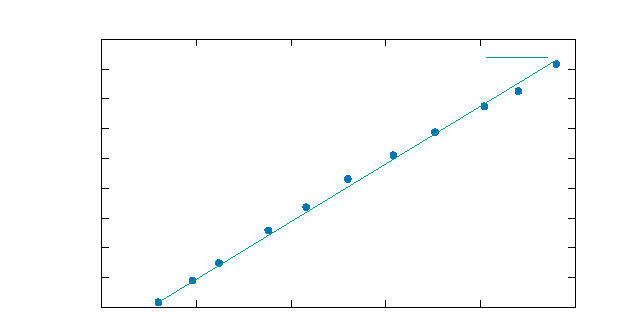
\includegraphics[width={288.00bp},height={144.00bp}]{zesileni}}%
    \gplfronttext
  \end{picture}%
\endgroup

    \captionsetup{type=graph}
    \caption{Závislost amplitud výstupního napětí na vstupním}
\end{figure}

\section{Závěr}

Změřil vstupní a výstupní charakteristiku tranzistoru v pracovním bodě $ (U_{D0}, U_{G0}) = ( 10 \ V, 3.6 \ V ) $ a dopočítal vnitřní odpor $ R_i = 18.9 \pm 2.8 \ \text{k}\Omega $ a statickou strmost $ S = 0.0617 \pm 0.0041 \ \Omega^{-1} $. Tyto hodnoty jsem potom použil při sestavováni zesilovače napětí, na kterém jsem měřil zesílení střídavého signálu $ A_M = A_M = 77.5 \pm 0.6 $. Tato hodnota dobře odpovídá zesílení určeného z charakteristik $ A_G = 80.5 \pm 2 $ a $ A_V = 78 \pm 4 $.
   
   

\begin{thebibliography}{0}
\bibitem{tabulky} Návod k úloze~\url{https://www.physics.muni.cz/praktika/static/navody/fp2/uloha02.pdf}.   
\end{thebibliography}

\end{document}
